% THIS DOCUMENT IS TAILORED TO REQUIREMENTS FOR SCIENTIFIC COMPUTING.  IT SHOULDN'T
% BE USED FOR NON-SCIENTIFIC COMPUTING PROJECTS
\documentclass[12pt]{article}

\usepackage{amsmath, mathtools}
\usepackage{amsfonts}
\usepackage{amssymb}
\usepackage{graphicx}
\usepackage{colortbl}
\usepackage{xr}
\usepackage{hyperref}
\usepackage{longtable}
\usepackage{xfrac}
\usepackage{tabularx}
\usepackage{float}
\usepackage{siunitx}
\usepackage{booktabs}
\usepackage{caption}
\usepackage{pdflscape}
\usepackage{afterpage}

\usepackage[round]{natbib}

%\usepackage{refcheck}

\hypersetup{
    bookmarks=true,         % show bookmarks bar?
      colorlinks=true,       % false: boxed links; true: colored links
    linkcolor=red,          % color of internal links (change box color with linkbordercolor)
    citecolor=green,        % color of links to bibliography
    filecolor=magenta,      % color of file links
    urlcolor=cyan           % color of external links
}

%% Comments

\usepackage{color}

\newif\ifcomments\commentstrue %displays comments
%\newif\ifcomments\commentsfalse %so that comments do not display

\ifcomments
\newcommand{\authornote}[3]{\textcolor{#1}{[#3 ---#2]}}
\newcommand{\todo}[1]{\textcolor{red}{[TODO: #1]}}
\else
\newcommand{\authornote}[3]{}
\newcommand{\todo}[1]{}
\fi

\newcommand{\wss}[1]{\authornote{blue}{SS}{#1}} 
\newcommand{\plt}[1]{\authornote{magenta}{TPLT}{#1}} %For explanation of the template
\newcommand{\an}[1]{\authornote{cyan}{Author}{#1}}

%% Common Parts

\newcommand{\progname}{ProgName} % PUT YOUR PROGRAM NAME HERE
\newcommand{\authname}{Team \#, Team Name
\\ Student 1 name
\\ Student 2 name
\\ Student 3 name
\\ Student 4 name} % AUTHOR NAMES                  

\usepackage{hyperref}
    \hypersetup{colorlinks=true, linkcolor=blue, citecolor=blue, filecolor=blue,
                urlcolor=blue, unicode=false}
    \urlstyle{same}
                                


% For easy change of table widths
\newcommand{\colZwidth}{1.0\textwidth}
\newcommand{\colAwidth}{0.13\textwidth}
\newcommand{\colBwidth}{0.82\textwidth}
\newcommand{\colCwidth}{0.1\textwidth}
\newcommand{\colDwidth}{0.05\textwidth}
\newcommand{\colEwidth}{0.8\textwidth}
\newcommand{\colFwidth}{0.17\textwidth}
\newcommand{\colGwidth}{0.5\textwidth}
\newcommand{\colHwidth}{0.28\textwidth}

% Used so that cross-references have a meaningful prefix
\newcounter{defnum} %Definition Number
\newcommand{\dthedefnum}{GD\thedefnum}
\newcommand{\dref}[1]{GD\ref{#1}}
\newcounter{datadefnum} %Datadefinition Number
\newcommand{\ddthedatadefnum}{DD\thedatadefnum}
\newcommand{\ddref}[1]{DD\ref{#1}}
\newcounter{theorynum} %Theory Number
\newcommand{\tthetheorynum}{TM\thetheorynum}
\newcommand{\tref}[1]{TM\ref{#1}}
\newcounter{tablenum} %Table Number
\newcommand{\tbthetablenum}{TB\thetablenum}
\newcommand{\tbref}[1]{TB\ref{#1}}
\newcounter{assumpnum} %Assumption Number
\newcommand{\atheassumpnum}{A\theassumpnum}
\newcommand{\aref}[1]{A\ref{#1}}
\newcounter{constraintnum} %Constraint Number
\newcommand{\rconstraintnum}{C\constraintnum}
\newcommand{\Cref}[1]{C\ref{#1}}
\newcounter{goalnum} %Goal Number
\newcommand{\gthegoalnum}{GS\thegoalnum}
\newcommand{\gsref}[1]{GS\ref{#1}}
\newcounter{instnum} %Instance Number
\newcommand{\itheinstnum}{IM\theinstnum}
\newcommand{\iref}[1]{IM\ref{#1}}
\newcounter{reqnum} %Requirement Number
\newcommand{\rthereqnum}{R\thereqnum}
\newcommand{\rref}[1]{R\ref{#1}}
\newcounter{frnum} %FR Number
\newcommand{\rthefrnum}{FR\thefrnum} 
\newcommand{\frref}[1]{FR\ref{#1}}
\newcounter{nfrnum} %NFR Number
\newcommand{\rthenfrnum}{NFR\thenfrnum}
\newcommand{\nfrref}[1]{NFR\ref{#1}}

\newcounter{lcnum} %Likely change number
\newcommand{\lthelcnum}{LC\thelcnum}
\newcommand{\lcref}[1]{LC\ref{#1}}

\newcounter{ulcnum} %Unlikely change number
\newcommand{\ltheulcnum}{ULC\theulcnum}
\newcommand{\ulcref}[1]{ULC\ref{#1}}

\usepackage{fullpage}

\newcommand{\deftheory}[9][Not Applicable]
{
\newpage
\noindent \rule{\textwidth}{0.5mm}

\paragraph{RefName: } \textbf{#2} \phantomsection 
\label{#2}

\paragraph{Label:} #3

\noindent \rule{\textwidth}{0.5mm}

\paragraph{Equation:}

#4

\paragraph{Description:}

#5

\paragraph{Notes:}

#6

\paragraph{Source:}

#7

\paragraph{Ref.\ By:}

#8

\paragraph{Preconditions for \hyperref[#2]{#2}:}
\label{#2_precond}

#9

\paragraph{Derivation for \hyperref[#2]{#2}:}
\label{#2_deriv}

#1

\noindent \rule{\textwidth}{0.5mm}

}

\begin{document}

\title{Software Requirements Specification \\ \textit{\progname: Smart Budgeting Expense Tracker}} 
\author{\authname}
\date{\today}
	
\maketitle

~\newpage

\pagenumbering{roman}

\tableofcontents

~\newpage

\section*{Revision History}

\begin{tabularx}{\textwidth}{p{3cm}p{2cm}X}
\toprule {\bf Date} & {\bf Version} & {\bf Notes}\\
\midrule
10/07/2024 & 1.0 & Added in the following sections to the SRS: Reference Materials (1), NFRs (5.2), Likely Changes (6), Unlikely Changes (7), Development Plan (9), Auxiliary Constraints (10)\\
10/08/2024 & 1.1 & Added in the following sections to the SRS: Purpose of Document (2.1), Organization of Document (2.4), User Characteristics (3.2)\\
10/09/2024 & 1.2 & Added in the following sections to the SRS: Characteristics of Intended Reader (2.3), Functional Requirements (5.1)\\
10/10/2024 & 1.3 & Added in the following sections to the SRS: System Constraints (3.3), Requirements Rationale (5.3)\\
\bottomrule 
\end{tabularx}

~\\
\plt{This template is intended for use by CAS 741.  For CAS 741 the template
should be used exactly as given, except the Reflection Appendix can be deleted.
For the capstone course it is a source of ideas, but shouldn't be followed
exactly.  The exception is the reflection appendix.  All capstone SRS documents
should have a refelection appendix.}

~\newpage

\section{Reference Material}

This section records information for easy reference.

\subsection{Table of Units}

N/A; units are not used in this SRS.

\subsection{Table of Symbols}

N/A; symbols are not used in this SRS.

\subsection{Abbreviations and Acronyms}

\renewcommand{\arraystretch}{1.2}
\begin{tabular}{l l} 
  \toprule		
  \textbf{symbol} & \textbf{description}\\
  \midrule 
  NLP & Natural Language Processing\\
  OCR & Optical Character Recognition\\
  JWT & JSON Web Token\\
  AI & Artificial Intelligence\\
  ML & Machine Learning\\
  LC & Likely Change\\
  ULC & Unlikely Change\\
  SRS & Software Requirements Specification\\
  TM & Theoretical Model\\
  \progname{} & \plt{put an expanded version of your program name here (as appropriate)}\\
  \bottomrule
\end{tabular}\\

\subsection{Mathematical Notation}

N/A; mathematical notation is not used in this SRS.

\newpage

\pagenumbering{arabic}

\plt{This SRS template is based on \citet{SmithAndLai2005, SmithEtAl2007,
  SmithAndKoothoor2016}.  It will get you started.  You should not modify the
  section headings, without first discussing the change with the course
  instructor.  Modification means you are not following the template, which
  loses some of the advantage of a template, especially standardization.
  Although the bits shown below do not include type information, you may need to
  add this information for your problem.  If you are unsure, please can ask the
  instructor.}

\plt{Feel free to change the appearance of the report by modifying the LaTeX
  commands.}

\plt{This template document assumes that a single program is being documented.
  If you are documenting a family of models, you should start with a commonality
  analysis.  A separate template is provided for this.  For program
  families you should look at \cite{Smith2006, SmithMcCutchanAndCarette2017}.
  Single family member programs are often programs based on a single physical
  model.  General purpose tools are usually documented as a family.  Families of
  physical models also come up.}

\plt{The SRS is not generally written, or read, sequentially.  The SRS is a
  reference document.  It is generally read in an ad hoc order, as the need
  arises.  For writing an SRS, and for reading one for the first time, the
  suggested order of sections is:
\begin{itemize}
\item Goal Statement
\item Instance Models
\item Requirements
\item Introduction
\item Specific System Description
\end{itemize}
}

\plt{Guiding principles for the SRS document:
\begin{itemize}
\item Do not repeat the same information at the same abstraction level.  If
  information is repeated, the repetition should be at a different abstraction
  level.  For instance, there will be overlap between the scope section and the
  assumptions, but the scope section will not go into as much detail as the
  assumptions section.
\end{itemize}
}

\plt{The template description comments should be disabled before submitting this
  document for grading.}

\plt{You can borrow any wording from the text given in the template.  It is part
  of the template, and not considered an instance of academic integrity.  Of
  course, you need to cite the source of the template.}

\plt{When the documentation is done, it should be possible to trace back to the
  source of every piece of information.  Some information will come from
  external sources, like terminology.  Other information will be derived, like
  General Definitions.}

\plt{An SRS document should have the following qualities: unambiguous,
  consistent, complete, validatable, abstract and traceable.}

\plt{The overall goal of the SRS is that someone that meets the Characteristics
  of the Intended Reader (Section~\ref{sec_IntendedReader}) can learn,
  understand and verify the captured domain knowledge.  They should not have to
  trust the authors of the SRS on any statements.  They should be able to
  independently verify/derive every statement made.}

\section{Introduction}

\plt{The introduction section is written to introduce the problem.  It starts
  general and focuses on the problem domain. The general advice is to start with
a paragraph or two that describes the problem, followed by a ``roadmap''
paragraph.  A roadmap orients the reader by telling them what sub-sections to
expect in the Introduction section.}

\subsection{Purpose of Document}

The purpose of this SRS document is to describe the functional and non-functional requirements of the Plutos budgeting application. This document serves as a formal agreement between stakeholders, including developers, project managers, and end users, to ensure a shared understanding of the system's objectives, capabilities, and constraints. \\

\noindent The SRS defines the expectations for the project, detailing the system features, behaviour, and performance requirements. It serves as a reference throughout the development lifecycle, guiding the design, implementation, testing, and validation phases to ensure the final product meets the agreed-upon specifications. Additionally, this document will support future maintenance and scalability of the application by providing clear and detailed requirements that facilitate ongoing enhancements.

\subsection{Scope of Requirements} 

The scope of this project encompasses the development of a budgeting application, Plutos, that automates expense tracking 
and categorization using AI. The system is designed to address key pain points for young adults struggling to manage their 
finances, specifically focusing on automating the process of tracking spending through receipt scanning, categorization of 
expenses, providing metrics to users regarding their spending habits, and providing feedback on how users can meet their 
budgeting goals.\\

\noindent However, some features that are outside the scope of the project (though may be implemented later) are: 

\begin{itemize}
  \item The system will not account for complex financial scenarios such as investments, stock portfolios, or retirement planning.
  \item Advanced financial forecasting or predictive analytics beyond simple budgeting trends will not be implemented.
  \item The AI model will not handle non-standard or highly complex receipts (e.g., multi-page invoices or handwritten receipts).
  \item The application will not offer integration with external financial accounts such as credit cards or bank accounts.
  \item The model will be trained to detect receipt data from Fortinos and will not initially support various receipt formats.
\end{itemize}

\noindent These exclusions allow the project to concentrate on core features, such as receipt scanning and expense categorization, while ensuring a manageable scope for the development process.

\subsection{Characteristics of Intended Reader} \label{sec_IntendedReader}
The primary audience for this SRS document is the group of undergraduate software engineering students who will 
oversee and complete the project’s design and implementation. This group of specialists, which includes system architects, 
software developers, and quality assurance testers, has extensive experience in the range of technologies needed for 
the project. Through their coursework and personal experiences, they are familiar with the process of developing mobile 
applications, and as they move through the project milestones, they will deepen their understanding of artificial intelligence 
and machine learning. They will actively learn how to apply AI/ML technologies in real-world circumstances throughout 
the project, which will advance their development as software engineers. The collaborative effort will help them improve 
their real-world application development abilities as the project progresses through seven milestones, ensuring that they 
are prepared to produce a practical and user-friendly budgeting solution.
\subsection{Organization of Document}

The following sections of the SRS will further describe the system and its requirements. The sections will be as follows:

\begin{enumerate}
	\setcounter{enumi}{2}
	\item General System Description
	\item Specific System Description
	\item Requirements
	\item Likely Changes
	\item Unlikely Changes
	\item Traceability Matrices and Graphs
	\item Development Plan
	\item Values of Auxiliary Constants
\end{enumerate}

\newpage

\section{General System Description}

This section provides general information about the system.  It identifies the
interfaces between the system and its environment, describes the user
characteristics and lists the system constraints.  \plt{This text can likely be
  borrowed verbatim.}

\plt{The purpose of this section is to provide general information about the
  system so the specific requirements in the next section will be easier to
  understand. The general system description section is designed to be
  changeable independent of changes to the functional requirements documented in
  the specific system description. The general system description provides a
  context for a family of related models.  The general description can stay the
  same, while specific details are changed between family members.}

\subsection{System Context}

\begin{figure}[h!]
  \centering
   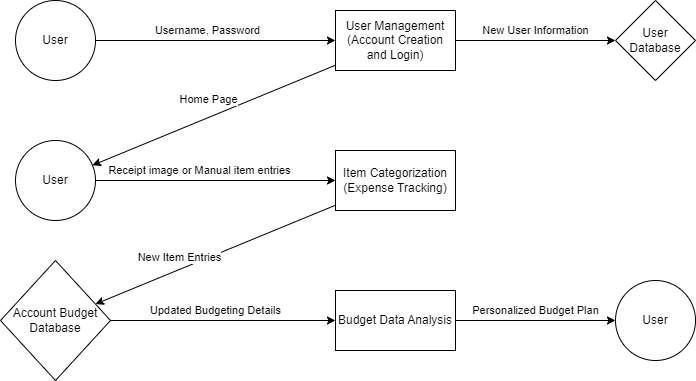
\includegraphics[width=\textwidth]{SystemContext.png}
  \caption{System Context}
  \label{Fig_SystemContext} 
\end{figure}

The system context for this project consists of a user(s), an expense tracking system, 
a budgeting analysis generator, and several databases. The user provides expense 
tracking inputs, such as physical/digital receipts or manual expense entries, and 
receives financial assessments. The expense tracking system processes user inputs, 
generates budgetary evaluations, and interacts with the financial analysis program 
and databases. The expense tracking system is also responsible for ensuring the 
validity of all inputs and provides a response if an invalid input is identified. 
The budgeting analysis generator provides expense categorization and evaluation 
functionalities, such as data analysis and visualization, and supports the expense 
tracking system in generating outputs. The database will be used to store user 
account information, user budget data, and supports the expense tracking system 
in storing and retrieving specific items and their respective categories. 
The system will typically be used for personal finance management, budgeting, 
and expense tracking, and may also be used for educational purposes. While 
the system is not safety-critical, it is important to ensure that the system is 
reliable and accurate in its calculations and analysis to provide users with 
trustworthy insights into their financial situation.



\plt{Your system context will include a figure that shows the abstract view of
  the software.  Often in a scientific context, the program can be viewed
  abstractly following the design pattern of Inputs $\rightarrow$ Calculations
  $\rightarrow$ Outputs.  The system context will therefore often follow this
  pattern.  The user provides inputs, the system does the calculations, and then
  provides the outputs to the user.  The figure should not show all of the
  inputs, just an abstract view of the main categories of inputs (like material
  properties, geometry, etc.).  Likewise, the outputs should be presented from
  an abstract point of view.  In some cases the diagram will show other external
  entities, besides the user.  For instance, when the software product is a
  library, the user will be another software program, not an actual end user.
  If there are system constraints that the software must work with external
  libraries, these libraries can also be shown on the System Context diagram.
  They should only be named with a specific library name if this is required by
  the system constraint.}

\begin{figure}[h!]
\begin{center}
 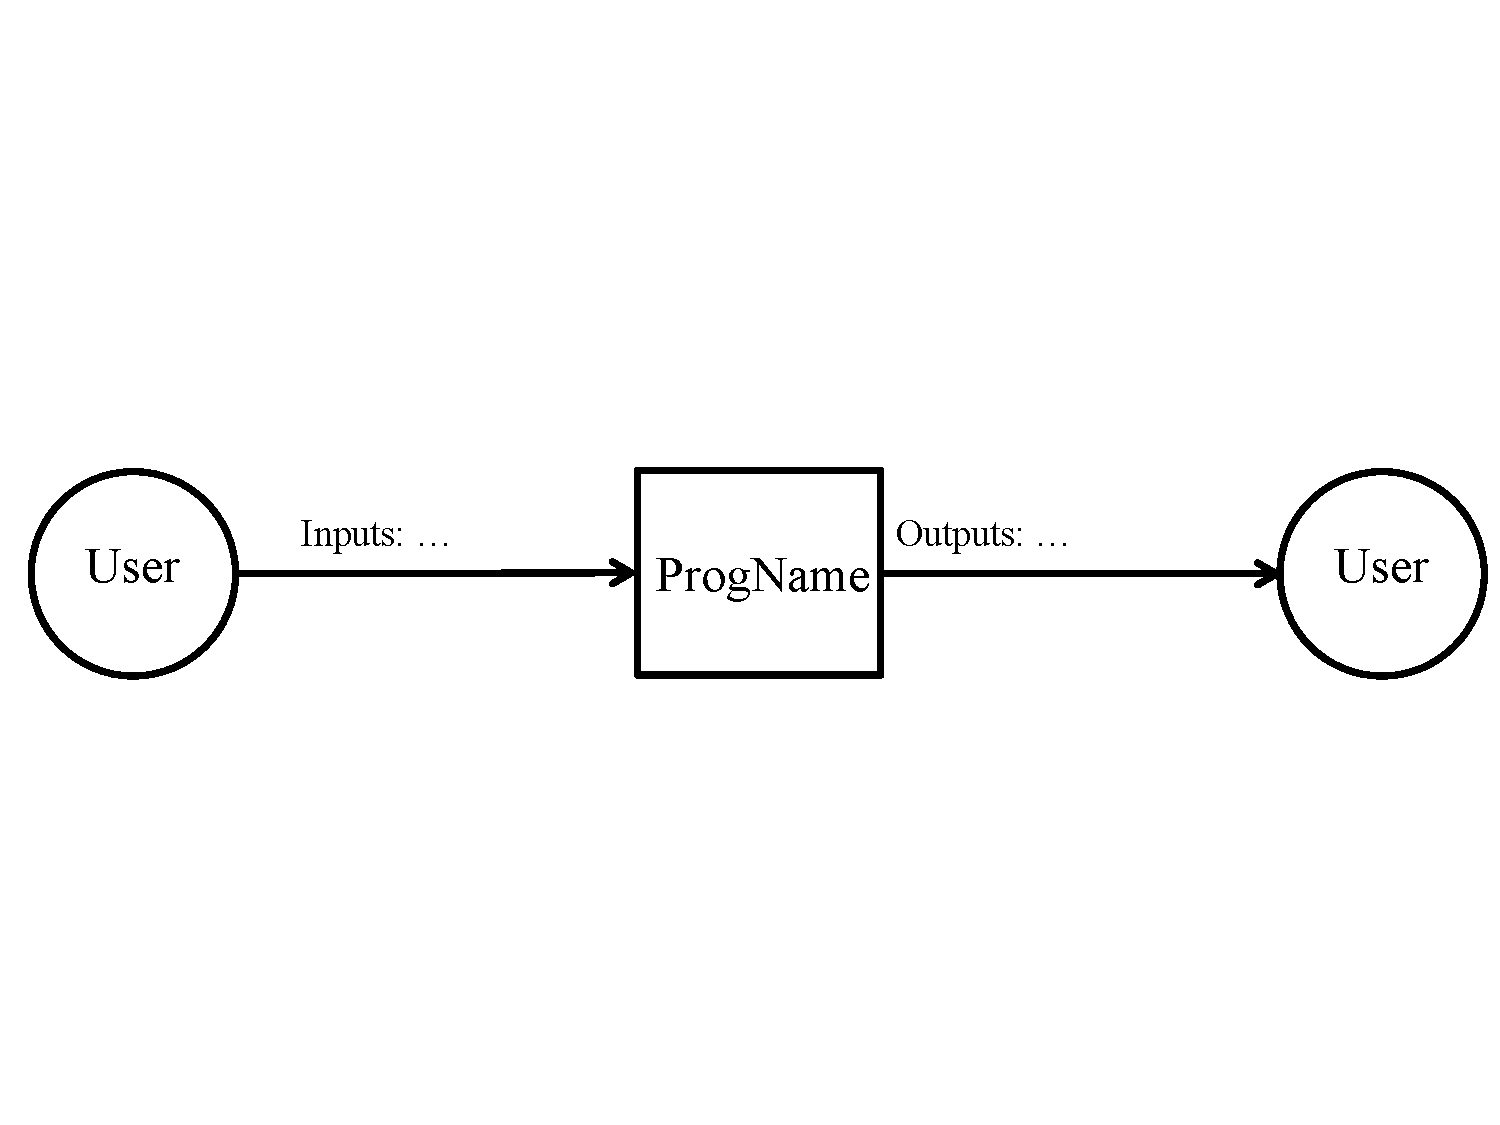
\includegraphics[width=0.6\textwidth]{SystemContextFigure}
\caption{System Context}
\label{Fig_SystemContext} 
\end{center}
\end{figure}

\plt{For each of the entities in the system context diagram its responsibilities
  should be listed.  Whenever possible the system should check for data quality,
  but for some cases the user will need to assume that responsibility.  The list
  of responsibilities should be about the inputs and outputs only, and they
  should be abstract.  Details should not be presented here.  However, the
  information should not be so abstract as to just say ``inputs'' and
  ``outputs''.  A summarizing phrase can be used to characterize the inputs.
  For instance, saying ``material properties'' provides some information, but it
  stays away from the detail of listing every required properties.}

\begin{itemize}
\item User Responsibilities:
\begin{itemize}
\item 
\end{itemize}
\item \progname{} Responsibilities:
\begin{itemize}
\item Detect data type mismatch, such as a string of characters instead of a
  floating point number
\item 
\end{itemize}
\end{itemize}

\plt{Identify in what context the software will typically be used.  Is it for
exploration? education? engineering work? scientific work?. Identify whether it
will be used for mission-critical or safety-critical applications.} \plt{This
additional context information is needed to determine how much effort should be
devoted to the rationale section.  If the application is safety-critical, the
bar is higher.  This is currently less structured, but analogous to, the idea to
the Automotive Safety Integrity Levels (ASILs) that McSCert uses in their
automotive hazard analyses.}

\wss{The }
\subsection{User Characteristics} \label{SecUserCharacteristics}

The users of the \textit{Plutos} budgeting application can be grouped into four main categories based on their financial experience and needs. These groups represent varying levels of financial literacy and desired interaction with budgeting tools.

\begin{enumerate}
	\item \textbf{First and Second-Year Undergraduate Students [Primary]} \\ 
		This group consists of young adults who are new to managing their finances independently, such as those living away from home for the first time. The characteristics of these users are as follows:
		\begin{itemize}
			\item \textbf{Financial Knowledge:} Limited experience with budgeting, managing expenses like rent and groceries. Usually have limited financial independence.
			\item \textbf{Time Management:} Busy schedules juggling school, work, and social commitments. Likely to prefer simple, intuitive interfaces that reduce time spent on budgeting.
			\item \textbf{Pain Points:} Lack of education on budgeting, potential to overspend due to unfamiliarity with managing day-to-day expenses.
		\end{itemize}
	\item \textbf{Upper-Year Undergraduate and Post-Graduate Students [Secondary]}
		This group includes more experienced students who have more financial independence as they have had experience managing their finances (in previous years living independently).  They have a better understanding of budgeting and have developed more mature spending habits.
		\begin{itemize}
			\item \textbf{Financial Knowledge:}  Some experience balancing school and work, likely to have a clearer understanding of budgeting needs and differentiating between wants and needs.
			\item \textbf{Time Management:} Likely to have more experience managing limited time and money, though they may still struggle with large financial decisions such as housing or loans.
			\item \textbf{Pain Points:}  May underestimate or overestimate budget needs, particularly with larger expenses.
		\end{itemize}
	\item \textbf{Early Career Professionals [Tertiary]}
		New graduates or individuals recently introduced to the workforce fall into this category. They likely have more stable incomes and financial independence.
		\begin{itemize}
			\item \textbf{Financial Knowledge:} More knowledgeable about saving, budgeting, and managing recurring expenses but still learning to navigate significant financial decisions.
			\item \textbf{Time Management:} May experience stress due to work-related issues and life changes such as moving to a new city and budgeting/tracking expenses may be another stress inducer on top of the new environment.
			\item \textbf{Pain Points:} Struggles with planning for long-term financial goals or managing joint accounts with a partner.
		\end{itemize}
	\item \textbf{Retirees [Tertiary]}
		Although retirees are not a primary focus, they may use the application to simplify financial tracking and planning for a fixed income.
		\begin{itemize}
			\item \textbf{Financial Knowledge:} Likely to have extensive experience with financial management but may struggle to adapt to modern budgeting tools.
			\item \textbf{Time Management:} Older users may face physical limitations (e.g., difficulty typing or navigating) and slower adaptation to new technologies.
			\item \textbf{Pain Points:} Difficulty managing finances without a steady income and adapting to increased living expenses.
		\end{itemize}
\end{enumerate}

\newpage

\subsection{System Constraints}

\begin{itemize}
  \item [C\refstepcounter{constraintnum}\theconstraintnum :] \textbf{Technical Constraints}
    \begin{itemize}
      \item The system must be developed as a mobile application using a cross-platform framework (e.g., React Native, Flutter) to ensure compatibility with both iOS and Android devices.
      \item The system must utilize a cloud-based backend technology (e.g., AWS, Firebase) to provide scalability and reliability.
      \item The system must integrate with a third-party OCR library (e.g., Tesseract OCR, Google Vision API) to provide optical character recognition functionality.
      \item The system must use a NoSQL database (e.g., MongoDB, Firebase) to store user account information and expense tracking data.
    \end{itemize}

  \item [C\refstepcounter{constraintnum}\theconstraintnum :] \textbf{Performance Constraints} 
    \begin{itemize}
      \item The system must be able to process user inputs and generate budgeting data and analysis outputs within a reasonable time frame (e.g., 2-3 seconds). 
      \item The system must be able to handle a minimum of 10 concurrent users without significant performance degradation. 
    \end{itemize}

  \item [C\refstepcounter{constraintnum}\theconstraintnum :] \textbf{Security Constraints} 
    \begin{itemize} 
      \item The system must implement secure password storage and authentication mechanisms using a third-party authentication service (e.g., Auth0, Firebase). 
      \item The system must ensure that all data transmitted between the client and server is encrypted using SSL/TLS protocol. 
    \end{itemize}
  
  \item [C\refstepcounter{constraintnum}\theconstraintnum :] \textbf{Environmental Constraints} 
    \begin{itemize} 
      \item The system must be designed to operate on a variety of mobile devices, including smartphones and tablets, with different screen sizes and operating systems. 
      \item The system must be able to operate in a variety of network environments, including Wi-Fi, cellular networks, and offline mode. 
    \end{itemize}
  
  \item [C\refstepcounter{constraintnum}\theconstraintnum :] \textbf{Regulatory Constraints} 
    \begin{itemize} 
      \item The system must comply with relevant data protection regulations (e.g., GDPR, CCPA) to ensure the privacy and security of user data. 
      \item The system must comply with relevant financial regulations (e.g., PCI-DSS) to ensure the secure handling of financial information. 
    \end{itemize}
\end{itemize}

\plt{System constraints differ from other type of requirements because they
  limit the developers' options in the system design and they identify how the
  eventual system must fit into the world. This is the only place in the SRS
  where design decisions can be specified.  That is, the quality requirement for
  abstraction is relaxed here.  However, system constraints should only be
  included if they are truly required.}

\newpage

% ----------------
% SECTION 4
% ----------------
\section{Specific System Description}

This section first presents the problem description, which gives a high-level
view of the problem to be solved. Following this, a solution characteristics
specification is typically included; however this aspect is not applicable for
this SRS.


\subsection{Problem Description} \label{Sec_pd}

The problem description can be found in Section 1 of the
\href{https://github.com/PlutosCapstone/Plutos/blob/main/docs/ProblemStatementAndGoals/ProblemStatement.pdf}{Problem
Statements and Goals} document.

\subsubsection{Terminology and  Definitions}

This subsection provides a list of terms that are used in the subsequent
sections and their meaning, with the purpose of reducing ambiguity and making it
easier to correctly understand the requirements:

\begin{itemize}
  \item \textbf{User Database}: A secure storage location for user information,
  including usernames, passwords, and personal financial profiles.
  \item \textbf{Item Categorization}: The classification of expenses and income
  into distinct categories, such as groceries, rent, and salary, to clarify
  spending habits.
  \item \textbf{Expense Tracking}: The practice of recording and monitoring
  expenditures to understand spending patterns and make informed financial
  decisions.
  \item \textbf{Budget Data Analysis}: The examination of financial data related
  to budgets to identify trends, patterns, and areas for improvement.
  \item \textbf{Personalized Budget Plan}: A customized budget tailored to an
  individual's specific financial goals, income levels, and spending habits.
  \item \textbf{Account Budget Database}: A system for storing and managing
  users' budget data, including allocations, spending limits, and financial
  goals.
  \item \textbf{Digital Financial Tools}: Software applications designed to help
  users manage their finances, including budgeting, tracking expenses, and
  analyzing data.
  \item \textbf{Data Security}: Measures taken to protect personal financial
  information from unauthorized access or breaches.
  \item \textbf{User-Friendly Interface}: An application design that prioritizes
  ease of use and accessibility, making it simple for users to navigate
  financial tools.
\end{itemize}

\subsubsection{Physical System Description} \label{sec_phySystDescrip}

\textbf{PS1: User Interface Elements}
\begin{itemize}
  \item \textbf{Camera Interface}: A feature that enables users to capture
  images of receipts using their mobile device’s camera
  \item \textbf{Receipt Preview}: A visual display showing the captured receipt
  for user verification before processing
  \item \textbf{Categorization Display}: An interface that shows identified
  items along with suggested categories for each item
  \item \textbf{Forms}: Input fields for entering financial data, such as income
  and expenses
  \item \textbf{Graphs and Charts}: Visual representations of spending patterns
  and budget performance, providing insights into financial health
\end{itemize}

\noindent
\textbf{PS2: Data Processing Components}
\begin{itemize}
  \item \textbf{Budgeting Algorithm}: An engine that analyzes user data to
  suggest personalized budgets based on historical spending
  \item \textbf{Notification System}: A feature that alerts users about
  important financial events, such as nearing budget limits or upcoming bill
  payments
  \item \textbf{Optical Character Recognition (OCR)}: A technology that analyzes
  the scanned receipt image to extract text, identifying items, prices, and
  totals
  \item \textbf{Item Categorization Engine}: A module that automatically
  classifies extracted items into predefined categories (e.g., groceries,
  clothing, dining) based on user-defined rules or machine learning algorithms
  \item \textbf{Expense Tracker}: A feature that logs categorized items into the
  user’s financial records, updating their spending summaries
\end{itemize}

\noindent
\textbf{PS3: User Input and Interaction}
\begin{itemize}
  \item Users interact with the application by entering financial data, setting
  budgets, and reviewing visualizations. 
  \item The application responds by updating financial summaries and providing
  insights based on user behavior
\end{itemize}

\noindent
\textbf{PS4: External Interfaces}
\begin{itemize}
  \item The application may integrate with external services, such as bank
  account linking via APIs, allowing users to automatically import transactions
  for more accurate tracking
\end{itemize}

\noindent
\textbf{PS5: Boundary Conditions}
\begin{itemize}
  \item Security protocols to protect user data, including encryption and secure
  authentication methods
  \item Limits on budget categories and spending thresholds to encourage
  responsible financial behavior
\end{itemize}

\noindent
\textbf{PS6: Conceptual Interactions}
\begin{itemize}
  \item The relationship between user inputs and financial outputs (e.g., how
  changes in spending habits affect overall budget health)
  \item Feedback loops where users receive insights based on their financial
  decisions, influencing future behavior
\end{itemize}

\plt{The purpose of this section is to clearly and unambiguously state the
  physical system that is to be modelled. Effective problem solving requires a
  logical and organized approach. The statements on the physical system to be
  studied should cover enough information to solve the problem. The physical
  description involves element identification, where elements are defined as
  independent and separable items of the physical system. Some example elements
  include acceleration due to gravity, the mass of an object, and the size and
  shape of an object. Each element should be identified and labelled, with their
  interesting properties specified clearly. The physical description can also
  include interactions of the elements, such as the following: i) the
  interactions between the elements and their physical environment; ii) the
  interactions between elements; and, iii) the initial or boundary conditions.}

\plt{The elements of the physical system do not have to correspond to an actual
physical entity.  They can be conceptual.  This is particularly important when
the documentation is for a numerical method. }

The physical system of \progname{}, as shown in Figure~?, includes the following
elements:

\begin{itemize}

\item[PS1:] 

\item[PS2:] ...

\end{itemize}



\plt{A figure here makes sense for most SRS documents}

% \begin{figure}[h!] \begin{center} %\rotatebox{-90}
% {
%  \includegraphics[width=0.5\textwidth]{<FigureName>}
% }
% \caption{\label{<Label>} <Caption>} \end{center} \end{figure}

\subsubsection{Goal Statements}

The goal statements can be found in Section 2 of the
\href{https://github.com/PlutosCapstone/Plutos/blob/main/docs/ProblemStatementAndGoals/ProblemStatement.pdf}{Problem
Statement and Goals} document.

\newpage


\subsection{Solution Characteristics Specification}
This section is not applicable to the SRS; the solution characteristics are
defined through the functional and nonfunctional requirements in Section 5 of
this document.

\subsubsection{Types}
Not applicable.

\subsubsection{Scope Decisions}
Not applicable.

\subsubsection{Modelling Decisions}
Not applicable.

\subsubsection{Assumptions} \label{sec_assumpt} Not applicable.

\subsubsection{General Definitions}\label{sec_gendef} Not applicable.

\subsubsection{Data Definitions}\label{sec_datadef} Not applicable.

\subsubsection{Data Types}\label{sec_datatypes} Not applicable.

\subsubsection{Instance Models} \label{sec_instance}    
Not applicable.

\subsubsection{Input Data Constraints} \label{sec_DataConstraints}    
Not applicable.

\subsubsection{Properties of a Correct Solution} \label{sec_CorrectSolution} Not
applicable.


\newpage


% ----------------
% SECTION 5
% ----------------
\section{Requirements}

\plt{The requirements refine the goal statement.  They will make heavy use of
  references to the instance models.}

This section provides the functional requirements, the business tasks that the
software is expected to complete, and the nonfunctional requirements, the
qualities that the software is expected to exhibit.

\subsection{Functional Requirements}
\noindent
\begin{itemize}
  \item [FR\refstepcounter{frnum}\thefrnum :] \textbf{User Account Management}
    \begin{itemize}
      \item Users must create an account using a name, email address, and password.
      \item Users can update their information after account creation.
      \item Users must log in using their registered email and password.
    \end{itemize}
  
  \item [FR\refstepcounter{frnum}\thefrnum :] \textbf{Receipt Scanning Input}
    \begin{itemize}
      \item Users can take a picture of a receipt and upload it.
      \item The system displays a preview for confirmation or retaking.
    \end{itemize}

  \item [FR\refstepcounter{frnum}\thefrnum :] \textbf{Manual Receipt Input}
    \begin{itemize}
      \item Users can manually input receipt details such as date and items.
      \item The system validates the input to ensure required fields are completed.
    \end{itemize}

  \item [FR\refstepcounter{frnum}\thefrnum :] \textbf{Database Management}
    \begin{itemize}
      \item The system shall maintain a secure, account-specific database for storing identified products and their respective categories.
    \end{itemize}

  \item [FR\refstepcounter{frnum}\thefrnum :] \textbf{Item Recognition and Categorization}
    \begin{itemize}
      \item The system shall identify and display item names, quantities, and costs from the uploaded receipt image.
      \item The system shall sort the entered products into predefined categories.
      \item The system shall prompt the user to confirm identified items and their corresponding categories.
      \item The system shall allow the user to modify the name, quantity, price, and category of the identified items.
      \item The system shall save the extracted data from the receipt input and the image of the receipt to the user’s profile.    
    \end{itemize}

  \item [FR\refstepcounter{frnum}\thefrnum :] \textbf{Financial Tracking}
    \begin{itemize}
      \item The system shall generate an overview of the user's spending history, including total spending by item category and trends over time.
      \item Users shall be able to set up budgets for each spending category.
      \item Users shall be able to view their spending in relation to their set budgets.
      \item The system shall notify users when they reach 80\% of their set budget limit.
      \item The system shall notify users when they achieve specified savings goals.
    \end{itemize}

\end{itemize}
\noindent \begin{itemize}

\item[R\refstepcounter{reqnum}\thereqnum \label{R_Inputs}:] \plt{Requirements
    for the inputs that are supplied by the user.  This information has to be
    explicit.}

\item[R\refstepcounter{reqnum}\thereqnum \label{R_OutputInputs}:] \plt{It isn't
    always required, but often echoing the inputs as part of the output is a
    good idea.}

\item[R\refstepcounter{reqnum}\thereqnum \label{R_Calculate}:] \plt{Calculation
    related requirements.}

\item[R\refstepcounter{reqnum}\thereqnum \label{R_VerifyOutput}:]
  \plt{Verification related requirements.}

\end{itemize}
\plt{Every IM should map to at least one requirement, but not every requirement
  has to map to a corresponding IM.}


\newpage

\subsection{Nonfunctional Requirements}

\noindent \begin{itemize}

\item[NFR\refstepcounter{nfrnum}\thenfrnum \label{NFR_Accuracy}:] \textbf{Accuracy}
	\begin{itemize}
		\item \textbf{Receipt Parsing Accuracy:} The machine learning model must achieve at least 80\% accuracy in correctly identifying and extracting key information (e.g., item names, prices, dates) from receipts.
		\item \textbf{Data Categorization Precision:} The app should categorize expenses into predefined categories (e.g., groceries, utilities, entertainment) with at least 90\% precision to ensure users' financial data is correctly organized.
		\item \textbf{Currency Calculation Precision:} All monetary calculations (totals, budgets, currency conversions) must maintain a precision of up to 2 decimal places to ensure accurate financial reporting.
		\item \textbf{OCR Model Accuracy:} The optical character recognition (OCR) model must correctly recognize text from images of receipts with a minimum accuracy rate of 95\%, ensuring minimal manual corrections by users.
		\item \textbf{Expense Summation Accuracy:} The app must guarantee 100\% accuracy in summing up expenses, incomes, and savings across different periods and categories, ensuring no rounding or summation errors.
		\item \textbf{Data Sync Consistency:} If the app syncs data across multiple devices or platforms, it should ensure 100\% consistency of financial data across all instances with no discrepancies or delays.
	\end{itemize}

\newpage

\item[NFR\refstepcounter{nfrnum}\thenfrnum \label{NFR_Usability}:] \textbf{Usability}
\begin{itemize}
	\item \textbf{User Interface Simplicity:} The app must have a clean, intuitive, and easy-to-navigate interface, allowing users to perform common tasks (e.g., adding expenses, viewing budgets) within 2-3 clicks.
	\item \textbf{Onboarding Process:} New users should be able to complete the account setup and understand core app features within 5 minutes, with interactive tutorials and tooltips provided during the first use.
	\item \textbf{Responsive Design:} The app’s interface must be fully responsive, providing an optimal user experience across different devices (smartphones, tablets, desktops) and screen sizes without layout or performance issues.
	\item \textbf{Error Prevention and Recovery:} The app should provide clear, informative error messages, and guide users through corrective actions when incorrect input is detected. Users should be able to recover from errors (e.g., wrong data entry) with no more than 2 steps.
	\item \textbf{Task Completion Time:} Common user tasks, such as adding a new receipt or setting a budget limit, should be completable within 10 seconds on average, assuming all required information is readily available.
	\item \textbf{Minimal Cognitive Load:} Information displayed to users must be concise and relevant, minimizing the cognitive effort needed to understand their financial data. Only essential details should be shown on the main dashboard, with advanced options tucked under menus.
	\item \textbf{Performance:} The app must load within 2 seconds for all major screens and respond to user actions (e.g., adding an entry, generating a report) within 1 second to ensure a smooth and responsive experience.
\end{itemize}

\item[NFR\refstepcounter{nfrnum}\thenfrnum \label{NFR_Maintainability}:] \textbf{Maintainability}
\begin{itemize}
	\item \textbf{Continuous Integration (CI) Pipeline:} The project must implement a CI pipeline that automatically runs tests, checks code quality, and verifies builds with every commit, ensuring that code is always in a deployable state.
	\item \textbf{Backward Compatibility:} New releases must maintain backward compatibility with previous versions, ensuring that users can seamlessly update the app without experiencing disruptions in their data or workflows.
	\item \textbf{Dependency Management:} The system should use a dependency management tool (e.g., npm for JavaScript, pip for Python) to track external libraries, and dependencies must be regularly updated to prevent security vulnerabilities and maintain compatibility with new features.
	\item \textbf{Automated Unit Testing Coverage:} At least 80\% of the codebase must be covered by automated unit tests to ensure maintainability and minimize the risk of introducing bugs when making changes.
\end{itemize}

\item[NFR\refstepcounter{nfrnum}\thenfrnum \label{NFR_Portability}:] \textbf{Portability} 
\begin{itemize}
	\item \textbf{Cross-Platform Compatibility:} The software should be compatible with Android and iOS mobile devices running the latest software.
	\item \textbf{Cloud-Based Data Storage:} The app must use cloud-based storage solutions (e.g., AWS S3, Google Cloud Storage) for user data to allow seamless access across devices without data loss or duplication.
	\item \textbf{Use of Platform-Agnostic Technologies:} The app should be developed using platform-agnostic frameworks or languages (e.g., React Native, Flutter, or web-based technologies like HTML5) to ensure easy deployment across different operating systems.
	\item \textbf{Portable Data Formats:} All data must be stored in platform-independent formats (e.g., JSON, CSV) for easy transfer and compatibility between devices, databases, and systems.
	\item \textbf{API Compatibility:} Any external APIs or third-party services integrated into the app must support cross-platform usage, ensuring the app can access necessary services from any supported platform.
	\item \textbf{Minimal Platform-Specific Dependencies:} The app should minimize reliance on platform-specific features or libraries, ensuring that any platform-dependent code can easily be replaced or adapted when porting the app to a new environment.
\end{itemize}

\item[NFR\refstepcounter{nfrnum}\thenfrnum \label{NFR_Reuseability}:] \textbf{Reusability} 
\begin{itemize}
	\item \textbf{Component-Based Architecture:} The app must be developed using reusable components (e.g., UI components, API services), allowing those components to be easily reused across different parts of the app or in future projects.
	\item \textbf{Separation of Concerns:} The app must adhere to the principle of separation of concerns, ensuring that business logic, data access, and presentation layers are kept separate, allowing individual layers to be reused independently.
	\item \textbf{Reusable Libraries and Modules:} Common functionalities (e.g., receipt parsing, authentication, data validation) must be abstracted into reusable libraries or modules that can be shared across multiple applications or systems.
	\item \textbf{Reusable Design Assets:} Design elements (e.g., icons, typography, color schemes) should be created as reusable assets, ensuring they can be reused consistently across multiple projects or platforms.
\end{itemize}

\newpage

\item[NFR\refstepcounter{nfrnum}\thenfrnum \label{NFR_Understandability}:] \textbf{Understandability} 
\begin{itemize}
	\item \textbf{Clear Code Documentation:} All source code must be thoroughly documented using inline comments and external documentation (e.g., README files, docstrings) to ensure that developers can easily understand the purpose and behavior of code components.
	\item \textbf{Consistent Naming Conventions:} Variables, functions, classes, and modules must follow consistent and meaningful naming conventions (e.g., camelCase, snake\_case) that clearly describe their functionality and usage, making the code easier to understand.
	\item \textbf{User-Friendly Interface:} The app's user interface (UI) must be designed with simplicity and clarity in mind, using clear labels, icons, and tooltips to guide users through tasks such as adding expenses or reviewing their budgets, reducing confusion.
	\item \textbf{Logical Code Structure:} The app's codebase must be organized logically, with related files and components grouped together in well-defined directories, so developers can easily navigate and locate specific functionality.
	\item \textbf{Readable Code Formatting:} The code must follow industry-standard formatting guidelines (e.g., proper indentation, line length limits) to ensure that it remains readable and easy to follow, both for developers and code reviewers.
	\item \textbf{Clear Error Messages:} The app must provide clear, descriptive error messages (both for users and in logs) that explain the cause of an issue and provide actionable steps to resolve it, improving user and developer understanding.
	\item \textbf{Detailed API Documentation:} Any APIs developed for the app must include detailed and easy-to-understand documentation, describing available endpoints, request/response formats, and example usage scenarios, ensuring that developers can integrate with them easily.
	\item \textbf{Version Control Documentation:} All major changes to the codebase should be accompanied by clear commit messages and detailed changelogs, explaining the purpose of changes and their impact, helping future developers understand the evolution of the project.
	\item \textbf{User-Centric Terminology:} The language and terminology used throughout the app's UI must be aligned with the users' mental models and expectations, using non-technical and familiar terms to enhance understanding.
\end{itemize}

\end{itemize}

\newpage

\subsection{Rationale}

\subsubsection{Scope Decisions}
The scope decisions were made with the intention of ensuring that the app delivers value to its target audience while remaining manageable within development constraints. The app focuses on personal budgeting features, including receipt scanning, expense categorization, budget tracking, and financial analysis. \\

\noindent\textbf{Rationale:}
\begin{itemize}
    \item \textbf{User-Centered Design}: The scope focuses on features that users expect from a smart budgeting app, aligning with current market demands for personal finance tools that offer automation (e.g., receipt scanning) and financial insights.
    \item \textbf{Technical Feasibility}: The decision to include features like machine learning for receipt parsing is scoped within the team’s ability to implement using existing AI frameworks (e.g., OCR and NLP libraries).
    \item \textbf{Time and Resource Constraints}: By narrowing the scope to core personal finance features, the team ensures that the project can be completed within the specified timeline and budget, avoiding feature creep.
    \item \textbf{Single Currency Support at Launch}: Focusing on a single currency simplifies the design of financial calculations, data presentation, and reporting. Multi-currency support introduces complexity in areas such as exchange rate management, which can be deferred to a later phase.
    \item \textbf{No Offline Mode in the Initial Version}: Implementing an offline mode adds complexity to data synchronization and storage. By focusing on online features initially, the development team can ensure that the core functionalities (e.g., receipt scanning and expense categorization) perform optimally without additional constraints.
\end{itemize}

\subsubsection{Modeling Decisions}
The app’s architecture follows a modular, service-oriented design, with key components such as receipt scanning, expense categorization, and budgeting reports being developed as independent, reusable modules.\\

\noindent\textbf{Rationale:}
\begin{itemize}
    \item \textbf{Scalability}: A modular approach allows the app to scale more easily by isolating functionalities into distinct services (e.g., a dedicated service for expense categorization). This reduces interdependencies and facilitates future growth.
    \item \textbf{Maintainability}: Modular components are easier to update and test, as changes to one service do not necessarily impact others. This also allows the app to accommodate feature updates and bug fixes more efficiently.
    \item \textbf{Reusability}: By designing reusable components (e.g., UI elements, API services), the app can easily extend its capabilities or integrate with other systems in the future.
    \item \textbf{Use of JSON for Data Exchange}: JSON is lightweight, human-readable, and widely used for web and mobile applications. Its simplicity makes it ideal for transmitting structured data between the client and server, ensuring smooth communication with minimal overhead.
\end{itemize}

\subsubsection{Assumptions}
Several assumptions were made during the development and design process. These assumptions include the expectation that users will regularly scan receipts, that mobile users are the primary audience, and that financial data privacy is of utmost importance.\\

\noindent\textbf{Rationale:}
\begin{itemize}
    \item \textbf{Receipt Scanning}: The assumption that users will consistently scan receipts underpins the app’s core functionality. This assumption is based on trends observed in personal finance apps where automation is a key value proposition for users.
    \item \textbf{Mobile-First Audience}: It is assumed that the majority of users will access the app via mobile devices. This assumption is driven by the current dominance of mobile platforms for personal finance management, offering convenience and accessibility.
    \item \textbf{Privacy and Security}: The assumption that users expect high standards of data privacy and security informs the app’s adherence to regulations such as GDPR. Users handling sensitive financial data expect robust protection mechanisms.
    \item \textbf{Stable Internet Connection}: It is assumed that users will have access to a stable internet connection while using the app, especially for features that require cloud processing (e.g., receipt scanning, data syncing, and report generation).
    \item \textbf{Regular App Usage}: The assumption is that users will interact with the app on a regular basis (e.g., weekly or monthly), allowing the app to provide up-to-date financial insights and budgeting trends based on frequent input.
    \item \textbf{User Financial Literacy}: The app assumes a basic level of financial literacy among its users, meaning that they will be able to understand concepts like budgets, expenses, savings, and categories without extensive in-app education.
\end{itemize}

\subsubsection{Typical Values}
For certain features, typical values have been used to inform design and development, such as default budget categories, receipt parsing accuracy thresholds, and system performance benchmarks.\\

\noindent\textbf{Rationale:}
\begin{itemize}
    \item \textbf{Default Categories}: Common budgeting categories (e.g., groceries, utilities, transportation) are provided as default to simplify user onboarding and offer a familiar framework. These categories were selected based on industry standards and user behavior in similar apps.
    \item \textbf{Parsing Accuracy}: An accuracy threshold of 90\% for receipt parsing was established as the minimum acceptable standard, based on current machine learning capabilities and user expectations for automated processes.
    \item \textbf{Performance Benchmarks}: Typical values for system performance, such as load times of under 2 seconds for key operations (e.g., viewing reports), are set based on user experience research, ensuring that the app feels responsive and efficient.
    \item \textbf{Maximum Receipt Upload Size}: A limit of 5 MB per receipt ensures a balance between allowing high-resolution images for accurate OCR processing while keeping server storage and bandwidth requirements manageable. Users are encouraged to upload clear, focused images within this size limit.
    \item \textbf{User Transaction History Retention}: Storing up to 3 years of transaction history provides users with enough data to analyze long-term financial trends while limiting the storage requirements for each user. Older transactions could be archived or made available on demand.
    \item \textbf{Frequency of Budget Update Notifications}: Weekly budget update notifications help users stay on top of their spending without overwhelming them with too many alerts. Users are reminded to review their financial status regularly while avoiding notification fatigue.
    \item \textbf{Budget Category Limits}: Allowing up to 25 distinct budget categories provides users with enough flexibility to categorize their spending without overwhelming them with too many options. This value strikes a balance between personalization and simplicity.
\end{itemize}

\plt{Provide a rationale for the decisions made in the documentation.  Rationale
should be provided for scope decisions, modelling decisions, assumptions and
typical values.}

\newpage 

\section{Likely Changes}    

\noindent \begin{itemize}
	\item[LC\refstepcounter{lcnum}\thelcnum\label{Addition of New Features}:] \textbf{Addition of New Features:} Based on user feedback, it is likely that new features (e.g., budgeting goal tracking, automatic expense categorization, or financial analytics) will be added to enhance user experience.
	\item[LC\refstepcounter{lcnum}\thelcnum\label{User Interface Redesign}:] \textbf{User Interface Redesign:} As usability testing is conducted, it's likely that the UI will undergo several iterations to improve the overall user experience and incorporate user feedback.
	\item[LC\refstepcounter{lcnum}\thelcnum\label{Integration with New APIs}:] \textbf{Integration with New APIs:} The app may need to integrate with new financial data APIs (e.g., bank transaction retrieval services) to enhance functionality, requiring changes to the codebase.
	\item[LC\refstepcounter{lcnum}\thelcnum\label{Change in Tech Stack}:] \textbf{Change in Tech Stack:} If the team encounters difficulties with the current technology stack, such as performance or compatibility issues, a transition to new technologies (e.g., switching from React to Vue.js) is likely.
	\item[LC\refstepcounter{lcnum}\thelcnum\label{Performance Optimizations}:] \textbf{Performance Optimizations:} As the app scales, there may be a need for performance enhancements, such as optimizing database queries or implementing caching strategies.
	\item[LC\refstepcounter{lcnum}\thelcnum\label{Data Privacy Compliance Updates}:] \textbf{Data Privacy Compliance Updates:} Changes in legal requirements (e.g., GDPR, CCPA) may require updates to the app's data handling and privacy policies to ensure compliance.
	\item[LC\refstepcounter{lcnum}\thelcnum\label{Adjustment of User Roles and Permissions}:] \textbf{Adjustment of User Roles and Permissions:} Changes to user roles and permissions may occur as new features are added, requiring adjustments to the authentication and authorization system.
	\item[LC\refstepcounter{lcnum}\thelcnum\label{Updates to User Authentication Method}:] \textbf{Updates to User Authentication Method:} There may be a transition to a more secure authentication method (e.g., implementing two-factor authentication) based on user feedback and security best practices.
	\item[LC\refstepcounter{lcnum}\thelcnum\label{Feedback Mechanism for Users}:] \textbf{Feedback Mechanism for Users:} Adding a feedback mechanism within the app (e.g., surveys or feedback forms) to gather user insights and suggestions for improvements is likely, ensuring continuous enhancement of the app based on user needs.
\end{itemize}

\newpage

\section{Unlikely Changes}    

\noindent \begin{itemize}
	\item[ULC\refstepcounter{ulcnum}\theulcnum\label{Complete Rewrite of the App}:] \textbf{Complete Rewrite of the App:} A complete rewrite of the app's codebase is unlikely unless there are significant fundamental flaws that cannot be addressed through refactoring.
	\item[ULC\refstepcounter{ulcnum}\theulcnum\label{Change in Database Choice}:] \textbf{Change in Database Choice:} During the development phase, the initial database choice may need to change due to performance issues or scalability requirements (e.g., moving from SQLite to PostgreSQL or MongoDB).
	\item[ULC\refstepcounter{ulcnum}\theulcnum\label{Switching Platforms}:] \textbf{Switching Platforms:} Transitioning from a mobile-first approach to a purely desktop application is unlikely if the initial target audience is primarily mobile users.
	\item[ULC\refstepcounter{ulcnum}\theulcnum\label{Adopting a New Programming Language}:] \textbf{Adopting a New Programming Language:} Changing the programming language for the entire project (e.g., from JavaScript to Ruby) midway through development is unlikely due to the complexity and resource investment required.
	\item[ULC\refstepcounter{ulcnum}\theulcnum\label{Elimination of Existing Features}:] \textbf{Elimination of Existing Features:} Removing core features that are central to the app's purpose (e.g., expense tracking) is unlikely, as these are fundamental to user expectations and functionality.
	\item[ULC\refstepcounter{ulcnum}\theulcnum\label{Change in Target Audience}:] \textbf{Change in Target Audience:} A shift in the target audience (e.g., from personal budgeting to corporate finance management) is unlikely as it would require a fundamental reevaluation of the app's design and features.
	\item[ULC\refstepcounter{ulcnum}\theulcnum\label{Discontinuation of Data Storage}:] \textbf{Discontinuation of Data Storage:} Completely removing any form of data storage (e.g., opting for a stateless application) is unlikely, as the core functionality relies on data retention for budgeting purposes.
	\item[ULC\refstepcounter{ulcnum}\theulcnum\label{Pivot to a Social Networking Feature Set}:] \textbf{Pivot to a Social Networking Feature Set:} A major pivot to add social networking features (e.g., allowing users to connect with friends or share budgets) is unlikely, as it diverges from the core functionality of personal budgeting and may complicate the app's primary purpose.
\end{itemize}

\newpage

\section{Traceability Matrices and Graphs}

The purpose of the traceability matrices is to provide easy references on what
has to be additionally modified if a certain component is changed.  Every time a
component is changed, the items in the column of that component that are marked
with an ``X'' may have to be modified as well.  Table~\ref{Table:trace} shows the
dependencies of theoretical models, general definitions, data definitions, and
instance models with each other. Table~\ref{Table:R_trace} shows the
dependencies of instance models, requirements, and data constraints on each
other. Table~\ref{Table:A_trace} shows the dependencies of theoretical models,
general definitions, data definitions, instance models, and likely changes on
the assumptions.

\plt{You will have to modify these tables for your problem.}

\plt{The traceability matrix is not generally symmetric.  If GD1 uses A1, that
  means that GD1's derivation or presentation requires invocation of A1.  A1
  does not use GD1.  A1 is ``used by'' GD1.}

\plt{The traceability matrix is challenging to maintain manually.  Please do
  your best.  In the future tools (like Drasil) will make this much easier.}

\afterpage{
\begin{landscape}
\begin{table}[h!]
\centering
\begin{tabular}{|c|c|c|c|c|c|c|c|c|c|c|c|c|c|c|c|c|c|c|c|}
\hline
	& \aref{A_OnlyThermalEnergy}& \aref{A_hcoeff}& \aref{A_mixed}& \aref{A_tpcm}& \aref{A_const_density}& \aref{A_const_C}& \aref{A_Newt_coil}& \aref{A_tcoil}& \aref{A_tlcoil}& \aref{A_Newt_pcm}& \aref{A_charge}& \aref{A_InitTemp}& \aref{A_OpRangePCM}& \aref{A_OpRange}& \aref{A_htank}& \aref{A_int_heat}& \aref{A_vpcm}& \aref{A_PCM_state}& \aref{A_Pressure} \\
\hline
\tref{T_COE}        & X& & & & & & & & & & & & & & & & & & \\ \hline
\tref{T_SHE}        & & & & & & & & & & & & & & & & & & & \\ \hline
\tref{T_LHE}        & & & & & & & & & & & & & & & & & & & \\ \hline
\dref{NL}           & & X& & & & & & & & & & & & & & & & & \\ \hline
\dref{ROCT}         & & & X& X& X& X& & & & & & & & & & & & & \\ \hline
\ddref{FluxCoil}    & & & & & & & X& X& X& & & & & & & & & & \\ \hline
\ddref{FluxPCM}     & & & X& X& & & & & & X& & & & & & & & & \\ \hline
\ddref{D_HOF}       & & & & & & & & & & & & & & & & & & & \\ \hline
\ddref{D_MF}        & & & & & & & & & & & & & & & & & & & \\ \hline
\iref{ewat}         & & & & & & & & & & & X& X& & X& X& X& & & X \\ \hline
\iref{epcm}         & & & & & & & & & & & & X& X& & & X& X& X& \\ \hline
\iref{I_HWAT}       & & & & & & & & & & & & & & X& & & & & X \\ \hline
\iref{I_HPCM}       & & & & & & & & & & & & & X& & & & & X & \\ \hline
\lcref{LC_tpcm}     & & & & X& & & & & & & & & & & & & & & \\ \hline
\lcref{LC_tcoil}    & & & & & & & & X& & & & & & & & & & & \\ \hline
\lcref{LC_tlcoil}   & & & & & & & & & X& & & & & & & & & & \\ \hline
\lcref{LC_charge}   & & & & & & & & & & & X& & & & & & & & \\ \hline
\lcref{LC_InitTemp} & & & & & & & & & & & & X& & & & & & & \\ \hline
\lcref{LC_htank}    & & & & & & & & & & & & & & & X& & & & \\
\hline
\end{tabular}
\caption{Traceability Matrix Showing the Connections Between Assumptions and Other Items}
\label{Table:A_trace}
\end{table}
\end{landscape}
}

\begin{table}[h!]
\centering
\begin{tabular}{|c|c|c|c|c|c|c|c|c|c|c|c|c|c|c|c|c|c|c|c|c|c|c|c|}
\hline        
	& \tref{T_COE}& \tref{T_SHE}& \tref{T_LHE}& \dref{NL}& \dref{ROCT} & \ddref{FluxCoil}& \ddref{FluxPCM} & \ddref{D_HOF}& \ddref{D_MF}& \iref{ewat}& \iref{epcm}& \iref{I_HWAT}& \iref{I_HPCM} \\
\hline
\tref{T_COE}     & & & & & & & & & & & & & \\ \hline
\tref{T_SHE}     & & & X& & & & & & & & & & \\ \hline
\tref{T_LHE}     & & & & & & & & & & & & & \\ \hline
\dref{NL}        & & & & & & & & & & & & & \\ \hline
\dref{ROCT}      & X& & & & & & & & & & & & \\ \hline
\ddref{FluxCoil} & & & & X& & & & & & & & & \\ \hline
\ddref{FluxPCM}  & & & & X& & & & & & & & & \\ \hline
\ddref{D_HOF}    & & & & & & & & & & & & & \\ \hline
\ddref{D_MF}     & & & & & & & & X& & & & & \\ \hline
\iref{ewat}      & & & & & X& X& X& & & & X& & \\ \hline
\iref{epcm}      & & & & & X& & X& & X& X& & & X \\ \hline
\iref{I_HWAT}    & & X& & & & & & & & & & & \\ \hline
\iref{I_HPCM}    & & X& X& & & & X& X& X& & X& & \\
\hline
\end{tabular}
\caption{Traceability Matrix Showing the Connections Between Items of Different Sections}
\label{Table:trace}
\end{table}

\begin{table}[h!]
\centering
\begin{tabular}{|c|c|c|c|c|c|c|c|}
\hline
	& \iref{ewat}& \iref{epcm}& \iref{I_HWAT}& \iref{I_HPCM}& \ref{sec_DataConstraints}& \rref{R_RawInputs}& \rref{R_MassInputs} \\
\hline
\iref{ewat}            & & X& & & & X& X \\ \hline
\iref{epcm}            & X& & & X& & X& X \\ \hline
\iref{I_HWAT}          & & & & & & X& X \\ \hline
\iref{I_HPCM}          & & X& & & & X& X \\ \hline
\rref{R_RawInputs}     & & & & & & & \\ \hline
\rref{R_MassInputs}    & & & & & & X& \\ \hline
\rref{R_CheckInputs}   & & & & & X& & \\ \hline
\rref{R_OutputInputs}  & X& X& & & & X& X \\ \hline
\rref{R_TempWater}     & X& & & & & & \\ \hline 
\rref{R_TempPCM}       & & X& & & & & \\ \hline
\rref{R_EnergyWater}   & & & X& & & & \\ \hline
\rref{R_EnergyPCM}     & & & & X& & & \\ \hline
\rref{R_VerifyOutput}  & & & X& X& & & \\ \hline
\rref{R_timeMeltBegin} & & X& & & & & \\ \hline
\rref{R_timeMeltEnd}   & & X& & & & & \\ 
\hline
\end{tabular}
\caption{Traceability Matrix Showing the Connections Between Requirements and Instance Models}
\label{Table:R_trace}
\end{table}

The purpose of the traceability graphs is also to provide easy references on
what has to be additionally modified if a certain component is changed.  The
arrows in the graphs represent dependencies. The component at the tail of an
arrow is depended on by the component at the head of that arrow. Therefore, if a
component is changed, the components that it points to should also be
changed. Figure~\ref{Fig_ATrace} shows the dependencies of theoretical models,
general definitions, data definitions, instance models, likely changes, and
assumptions on each other. Figure~\ref{Fig_RTrace} shows the dependencies of
instance models, requirements, and data constraints on each other.

% \begin{figure}[h!]
% 	\begin{center}
% 		%\rotatebox{-90}
% 		{
% 			\includegraphics[width=\textwidth]{ATrace.png}
% 		}
% 		\caption{\label{Fig_ATrace} Traceability Matrix Showing the Connections Between Items of Different Sections}
% 	\end{center}
% \end{figure}


% \begin{figure}[h!]
% 	\begin{center}
% 		%\rotatebox{-90}
% 		{
% 			\includegraphics[width=0.7\textwidth]{RTrace.png}
% 		}
% 		\caption{\label{Fig_RTrace} Traceability Matrix Showing the Connections Between Requirements, Instance Models, and Data Constraints}
% 	\end{center}
% \end{figure}

\newpage

\section{Development Plan}

The development plan can be found \href{https://github.com/PlutosCapstone/Plutos/blob/main/docs/DevelopmentPlan/DevelopmentPlan.pdf}{here}. \\

\noindent Note that information in this document, especially regarding dates and deadlines, are subject to change and will be updated accordingly. \\

\noindent All functional requirements specified in Section 5.1 are intended for implementation. \\

\noindent Non-functional requirements specified in Section 5.2 are to be followed but may be subject to change or constraints. \\

\section{Values of Auxiliary Constants}

There are no symbolic parameters used in this report.

\newpage

\bibliographystyle {plainnat}
\bibliography {../../refs/References}

\newpage

\noindent \plt{The following is not part of the template, just some things to consider
  when filing in the template.}

\noindent \plt{Grammar, flow and \LaTeX advice:
\begin{itemize}
\item For Mac users \texttt{*.DS\_Store} should be in \texttt{.gitignore}
\item \LaTeX{} and formatting rules
\begin{itemize}
\item Variables are italic, everything else not, includes subscripts (link to
  document)
\begin{itemize}
\item \href{https://physics.nist.gov/cuu/pdf/typefaces.pdf}{Conventions}
\item Watch out for implied multiplication
\end{itemize}
\item Use BibTeX
\item Use cross-referencing
\end{itemize}
\item Grammar and writing rules
\begin{itemize}
\item Acronyms expanded on first usage (not just in table of acronyms)
\item ``In order to'' should be ``to''
\end{itemize}
\end{itemize}}

\noindent \plt{Advice on using the template:
\begin{itemize}
\item Difference between physical and software constraints
\item Properties of a correct solution means \emph{additional} properties, not
  a restating of the requirements (may be ``not applicable'' for your problem).
  If you have a table of output constraints, then these are properties of a
  correct solution.
\item Assumptions have to be invoked somewhere
\item ``Referenced by'' implies that there is an explicit reference
\item Think of traceability matrix, list of assumption invocations and list of
  reference by fields as automatically generatable
\item If you say the format of the output (plot, table etc), then your
  requirement could be more abstract
\end{itemize}
}

\newpage{}
\section*{Appendix --- Reflection}

\wss{Not required for CAS 741}

The information in this section will be used to evaluate the team members on the
graduate attribute of Lifelong Learning.  

The purpose of reflection questions is to give you a chance to assess your own
learning and that of your group as a whole, and to find ways to improve in the
future. Reflection is an important part of the learning process.  Reflection is
also an essential component of a successful software development process.  

Reflections are most interesting and useful when they're honest, even if the
stories they tell are imperfect. You will be marked based on your depth of
thought and analysis, and not based on the content of the reflections
themselves. Thus, for full marks we encourage you to answer openly and honestly
and to avoid simply writing ``what you think the evaluator wants to hear.''

Please answer the following questions.  Some questions can be answered on the
team level, but where appropriate, each team member should write their own
response:

\begin{enumerate}
  \item What went well while writing this deliverable? 
  \item What pain points did you experience during this deliverable, and how did
  you resolve them?
  \item How many of your requirements were inspired by speaking to your
  client(s) or their proxies (e.g. your peers, stakeholders, potential users)?
  \item Which of the courses you have taken, or are currently taking, will help
  your team to be successful with your capstone project.
  \item What knowledge and skills will the team collectively need to acquire to
  successfully complete this capstone project?  Examples of possible knowledge
  to acquire include domain specific knowledge from the domain of your
  application, or software engineering knowledge, mechatronics knowledge or
  computer science knowledge.  Skills may be related to technology, or writing,
  or presentation, or team management, etc.  You should look to identify at
  least one item for each team member.
  \item For each of the knowledge areas and skills identified in the previous
  question, what are at least two approaches to acquiring the knowledge or
  mastering the skill?  Of the identified approaches, which will each team
  member pursue, and why did they make this choice?
\end{enumerate}

\end{document}